% \documentclass[sigplan,10pt,nonacm]{acmart}\settopmatter{printfolios=true,printccs=false,printacmref=false}

%% For double-blind review submission, w/o CCS and ACM Reference (max submission space)
% \documentclass[sigplan,review,anonymous]{acmart}\settopmatter{printfolios=true,printccs=false,printacmref=false}
%% For double-blind review submission, w/ CCS and ACM Reference
%\documentclass[sigplan,review,anonymous]{acmart}\settopmatter{printfolios=true}
%% For single-blind review submission, w/o CCS and ACM Reference (max submission space)
%\documentclass[sigplan,review]{acmart}\settopmatter{printfolios=true,printccs=false,printacmref=false}
%% For single-blind review submission, w/ CCS and ACM Reference
%\documentclass[sigplan,review]{acmart}\settopmatter{printfolios=true}
%% For final camera-ready submission, w/ required CCS and ACM Reference
\documentclass[sigplan,10pt]{acmart}\settopmatter{printfolios=true,printccs=false,printacmref=false}


%% Conference information
%% Supplied to authors by publisher for camera-ready submission;
%% use defaults for review submission.
\acmConference[Purdue CS590-DLS]{}{Dec 2019}{West Lafayette, Indiana}
\acmYear{2019}
\acmISBN{} % \acmISBN{978-x-xxxx-xxxx-x/YY/MM}
\acmDOI{} % \acmDOI{10.1145/nnnnnnn.nnnnnnn}
\startPage{1}


%% Copyright information
%% Supplied to authors (based on authors' rights management selection;
%% see authors.acm.org) by publisher for camera-ready submission;
%% use 'none' for review submission.
\setcopyright{none}
%\setcopyright{acmcopyright}
%\setcopyright{acmlicensed}
%\setcopyright{rightsretained}
%\copyrightyear{2018}           %% If different from \acmYear

%% Bibliography style
\bibliographystyle{ACM-Reference-Format}
%% Citation style
%\citestyle{acmauthoryear}  %% For author/year citations
%\citestyle{acmnumeric}     %% For numeric citations
%\setcitestyle{nosort}      %% With 'acmnumeric', to disable automatic
                            %% sorting of references within a single citation;
                            %% e.g., \cite{Smith99,Carpenter05,Baker12}
                            %% rendered as [14,5,2] rather than [2,5,14].
%\setcitesyle{nocompress}   %% With 'acmnumeric', to disable automatic
                            %% compression of sequential references within a
                            %% single citation;
                            %% e.g., \cite{Baker12,Baker14,Baker16}
                            %% rendered as [2,3,4] rather than [2-4].


%%%%%%%%%%%%%%%%%%%%%%%%%%%%%%%%%%%%%%%%%%%%%%%%%%%%%%%%%%%%%%%%%%%%%%
%% Note: Authors migrating a paper from traditional SIGPLAN
%% proceedings format to PACMPL format must update the
%% '\documentclass' and topmatter commands above; see
%% 'acmart-pacmpl-template.tex'.
%%%%%%%%%%%%%%%%%%%%%%%%%%%%%%%%%%%%%%%%%%%%%%%%%%%%%%%%%%%%%%%%%%%%%%


%% Some recommended packages.
\usepackage{booktabs}   %% For formal tables:
                        %% http://ctan.org/pkg/booktabs
\usepackage{subcaption} %% For complex figures with subfigures/subcaptions
                        %% http://ctan.org/pkg/subcaption
%% Some recommended packages.
\usepackage{booktabs}   %% For formal tables:
                        %% http://ctan.org/pkg/booktabs
\usepackage{subcaption} %% For complex figures with subfigures/subcaptions
                        %% http://ctan.org/pkg/subcaption
\usepackage[utf8]{inputenc}
\usepackage[T1]{fontenc}
\usepackage[scaled=0.8]{beramono}
\usepackage{amsmath}
\usepackage{amssymb}
\usepackage{booktabs}
\usepackage{xcolor,colortbl}
\usepackage{url}
\usepackage{listings}
\usepackage{paralist}
\usepackage{subcaption}
\usepackage{wrapfig}
\usepackage{enumitem}
\usepackage{multicol}
\usepackage{flushend}
\usepackage{bcprules}
\usepackage{nicefrac}
\usepackage{xfrac}
\usepackage{graphicx}
% ----- listings
%\definecolor{ckeyword}{HTML}{7F0055}
\definecolor{ckeyword}{HTML}{AE292A}
\definecolor{ccomment}{HTML}{3F7F5F}
\definecolor{cstring}{HTML}{2A0099}

\lstdefinelanguage{Scala}%
{morekeywords={abstract,%
  sealed,%
  case,catch,char,class,%
  def,else,extends,final,finally,for,%
  if,import,implicit,%
  match,module,%
  new,null,undefined,%
  fun,array,
  override,%
  package,private,protected,public,%
  for,public,return,super,%
  this,throw,trait,try,type,%
  val,var,%
  with,while,%
  let,skip,assert,then,fst,snd,root,idx,sum,prod,exists,forall,%
  yield,%
  letrec,lambda %add keywords for Scheme
  },%
  sensitive,%
  moredelim=*[il][\bfseries]{\#\#\ },
  morecomment=[l]//,%
  morecomment=[s]{/*}{*/},%
  morestring=[b]",%
%  morestring=[b]',%
  showstringspaces=false%
}[keywords,comments,strings]%

\lstset{language=Scala,%
  mathescape=true,%
%  columns=[c]fixed,%
%  basewidth={0.5em, 0.40em},%
%  aboveskip=5pt,%\smallskipamount,
%  belowskip=5pt,%\negsmallskipamount,
  lineskip=0pt,
  basewidth={0.54em, 0.4em},%
%  backgroundcolor=\color{listingbg},
  basicstyle=\footnotesize\ttfamily,
  keywordstyle=\keywordstyle,
  commentstyle=\commentstyle,
  stringstyle=\stringstyle,
%  xleftmargin=0.5cm
  literate={-->}{{$\to$}}3 
           {->}{{$\mapsto$}}3 
           {=>}{{$\Rightarrow$}}2 
           {|-}{{$\ts$}}2 
           %{fun}{{$\lambda$}}1 
           {∂}{{}}1 
           {idx}{{$\#$}}1 
           %{sum}{{$\Sigma$}}1 
           {array(}{{$\langle.\rangle$(}}3 
           %{[[}{{$[\![$}}1
           %{]]}{{$]\!]$}}1
           %{…}{{$\!...$}}1 
}

\definecolor{listingbg}{RGB}{240, 240, 240}

\newcommand{\commentstyle}[1]{\color{ccomment}\itshape{#1}}
%\newcommand{\keywordstyle}[1]{\color{ckeyword}\bfseries{#1}}
\newcommand{\keywordstyle}[1]{\color{ckeyword}{#1}}
\newcommand{\stringstyle}[1]{\color{cstring}\bfseries{#1}}

\lstnewenvironment{listing}{\lstset{language=Scala}}{}
\lstnewenvironment{listingtiny}{\lstset{language=Scala,basicstyle=\scriptsize\ttfamily}}{}

\newcommand{\code}[1]{\lstinline[language=Scala,columns=fixed,basicstyle=\ttfamily]|#1|}


\newcommand{\IMP}[0]{\texttt{IMP}}
\newcommand{\FUN}[0]{\texttt{FUN}}

\newcommand{\TOOL}[0]{\texttt{SIGMA}}



% ----- packed items, so we don't waste space
\newenvironment{sitemize}{
\begin{itemize}
  \setlength{\itemsep}{1pt}
  \setlength{\parskip}{0pt}
  \setlength{\parsep}{0pt}
}{\end{itemize}}

\newenvironment{senumerate}{
\begin{enumerate}
  \setlength{\itemsep}{1pt}
  \setlength{\parskip}{0pt}
  \setlength{\parsep}{0pt}
}{\end{enumerate}}

\newcommand{\mypar}[1]{{\bf #1.}}

% ----- formal

%\newcommand{\judgement}[2]{{\bf #1} \hfill #2}
%\newcommand{\den}[1]{$\left\llbracket$\;#1\;$\right\rrbracket$}
\newcommand{\den}[1]{\llbracket~#1~\rrbracket}

%\newcommand{\ts}{\,\vdash\,}
\newcommand{\evalsto}{\Downarrow}

\newcommand{\mbind}{\;{\small{\texttt{>>}\hspace{-0.3pt}\raisebox{-0.15pt}{\texttt{=}}}}\;}

%\newcommand{\mbind}{{\small{\texttt{>>}\hspace{-1.7pt}\raisebox{-0.15pt}{\texttt{=}}}}}

\newcommand{\rref}[1]{\textsc{(#1)}}

% ----- comments and todo

\newcommand{\note}[1]{{\color{red}[#1]}}
\newcommand{\todo}[1]{\note{TODO: #1}}

\newcommand{\silent}[1]{}



\begin{document}

%% Title information
\title{Learning Heuristics of SAT by Graph Neural Networks}         %% [Short Title] is optional;
                                        %% when present, will be used in
                                        %% header instead of Full Title.
%\titlenote{with title note}             %% \titlenote is optional;
                                        %% can be repeated if necessary;
                                        %% contents suppressed with 'anonymous'
% \subtitle{Subtitle}                     %% \subtitle is optional
% \subtitlenote{with subtitle note}       %% \subtitlenote is optional;
                                        %% can be repeated if necessary;
                                        %% contents suppressed with 'anonymous'

\author
[Guannan Wei]
{Guannan Wei \\ Purdue University}

\lstMakeShortInline[keywordstyle=,%
              flexiblecolumns=false,%
              %basewidth={0.56em, 0.52em},%
              mathescape=false,%
              basicstyle=\tt]@

%% Abstract
%% Note: \begin{abstract}...\end{abstract} environment must come
%% before \maketitle command
%\begin{abstract}
%\end{abstract}


%% 2012 ACM Computing Classification System (CSS) concepts
%% Generate at 'http://dl.acm.org/ccs/ccs.cfm'.
\begin{CCSXML}
<ccs2012>
<concept>
<concept_id>10011007.10011006.10011008</concept_id>
<concept_desc>Software and its engineering~General programming languages</concept_desc>
<concept_significance>500</concept_significance>
</concept>
<concept>
<concept_id>10003456.10003457.10003521.10003525</concept_id>
<concept_desc>Social and professional topics~History of programming languages</concept_desc>
<concept_significance>300</concept_significance>
</concept>
</ccs2012>
\end{CCSXML}

\ccsdesc[500]{Software and its engineering~General programming languages}
\ccsdesc[300]{Social and professional topics~History of programming languages}
%% End of generated code


%% Keywords
%% comma separated list
% \keywords{keyword1, keyword2, keyword3}  %% \keywords are mandatory in final camera-ready submission


%% \maketitle
%% Note: \maketitle command must come after title commands, author
%% commands, abstract environment, Computing Classification System
%% environment and commands, and keywords command.
\maketitle

\renewcommand\thefootnotecopyrightpermission{}
\footnotetextcopyrightpermission{Copyright held by the authors.}
\fancyhead[RO,LE]{Preprint, Dec 2019}

\section{Introduction}

In this paper, we report the progress and preliminary result on the CS590-DLS course project that aims 
to learn branching heuristics for the Boolean Satisfiability (SAT) problem based on DPLL algorithm. 

\paragraph{Background}

Given a formula consists of variables over booleans and propositional logic connectives, the satisfiability
problem asks an assignment, i.e., a mapping from variables to boolean values, that makes the formula be true. 
For example; $(P \wedge Q) \to (\neg Q \vee R)$ is a well-formed formula and can be satisfied by assigning
$P$ to be $\top$; $P \wedge \neg P$ is another well-formed formula but can not be satisfied, written as UNSAT.

A traditional approach to solve SAT is DPLL algorithm \cite{Davis:1962:MPT:368273.368557}. 
Although in the worst case, DPLL is still an exponential algorithm due the nature of the problem,
but on many instances DPLL is able to find a solution or prove UNSAT quickly.
Thus DPLL and its variants are widely used in many modern SAT solvers such as miniSAT.

The DPLL algorithm works on Conjunction Normal Form (CNF). 
A CNF formula is a conjunction of clauses. A clause is a disjunction of literals. 
A literal is either a variable (symbol) or a negation of a variable. 
Formulas in other forms can be translated to CNF \cite{tseitin1983complexity}. 
For example, $(x_1 \vee x_2) \wedge (\neg x_2 \vee x_3)$ is a well-formed formula in CNF.

With the CNF format introduced, now we can briefly describe the essential ideas behind DPLL: 
unit propagation, searching and backtracking.
If a clause contains only one literal, then it is a unit clause. Since the problem is given 
in CNF, this cluase is forced to be satisfied, thus we must assign this literal to be true. 
The unit propagation then calculate the consequential formula by making this assignment --
some clauses can be complete eliminated.
If the current formula does not contain an unit clause, the algorithm then chooses a branching
variable by predefined heuristics and assign either $\top$ or $\bot$ to this variable,
and then propagate this decision and recursively call the decision procedure.
At some point, we may reach a dead end that the current assignment shows an UNSAT result, 
then we need to recover to some previous decision we made and try another assignment.

The pseudocode of DPLL procedure is listed as follows:

\begin{lstlisting}
def dpll(f: Formula): Boolean = {
  if (f.hasUnsatClause) return false
  if (f.isSat) return true
  if (f.hasUnitClause) return dpll(f.elimUnitClause)
  val v = f.pickVariable
  val tryTrue = dpll(f.addUnitClause(v))
  if (tryTrue) true
  else dpll(f.addUnitClause(neg(v)))
}
\end{lstlisting}

Several variants based on this algorithm make it more efficient: 1) one can introduce
pure literal elimination, that is a variable appears with only one polarity can be 
assigned to a value that makes its containing clauses satisfies but without triggering
any conflict. 2) When we reach one dead end, we can perform a conflict analysis which 
produces a lemma that must be satisfied (known as conflict-driven clauses learning, CDCL
\cite{DBLP:series/faia/SilvaLM09}). 
The lemma will be added back to the formula, and the backtrack can be done in a non-chronological fashion.
In this paper, we constrain ourself to the simplest version of DPLL and focus on
learning how to choose the branching variable.

\paragraph{Problem Statement}

In the literatures, people have invented several efficient branching heuristics, 
from very simple ones such as picking the most frequent literal, 
to complicated ones such as such as VSIDS \cite{zhang2002quest}.
Literatures on branching heuristics can be found from \cite{hooker1995branching, li1997heuristics}.
But among these heuristics, no one works perfect for all kinds of instances.

The fundamental problem we are interested in is, given a such simple DPLL algorithm
framework, can we learn an efficient heuristics from scratch?
In this paper, we propose to use recent advances in graph neural networks to 
encode a CNF formula and use reinforcement learning to learn the branching heuristics.
We will use the policy gradient method for the reinforcement learning part.

\section{Model}

In this section, we briefly review the related work on graph representations of SAT
and then describe the model used in this paper.

\subsection{General Description}

\paragraph{Graph Representation}

The central problem on apply neural-network-based approach to SAT is how to 
represent a boolean formula and a decision in a differentiable way.
The formula can be easily represented by a sequence or a matrix, but this
representation losts the structural information and the invarant properties such as
exchange.
The graph neural networks have been applied to computational chemistry and 
social network analysis which also capture the permutation invariance and the 
structure of a CNF formula.
We first review NeuroSAT's graph embedding of a CNF formula \cite{selsam2018learning}.

Given a formula $F$ of $m$ clauses and $n$ variables in CNF, 
one can construct a graph $G = \langle V, E \rangle$ such that 
$V = V_{lit} \cup V_{cls}$ where $V_{lit}$ is the set of vertices that embed literals,
$V_{cls}$ is the set of vertices that embed clauses. 
And $E$ contains two different types of edge, the first one is the edegs that connect literals and its
containing clauses, the second type is the edges that connect a variable and its negation, formally,
$ E = \{ (l, c) | l \in c \} \cup \{ (l, \neg l) | l \}$ for all literals $l$ and clauses $c$.
Note that in the NeuroSAT's encoding, there is a vertex for every variable and its negation no matter
it appears or not, so the size of vertices set $|V| = 2n + m$.

\paragraph{Message-Passing Neural Network}

After the graph is constructed, NeuroSAT uses iterative message-passing mechanism to refine the 
vector space embeddings.
One iteration of a message-passing consists of two stages:
1) first every clause receives messages from its neighboring literals and update the clause embedding;
2) then every literal receives its message from its neighboring clauses and its negated literal vertices,
and update its embedding.

Suppose the size of embedding vectors is $d$. The initial embedding vectors of literals and clauses 
are $L^{0} \in \mathbb{R}^{2n \times d}$ and $C^{0} \in \mathbb{R}^{m \times d}$ which are randomly initialized.
NeuroSAT uses two MLPs $\mathcal{L}_{msg}$ and $\mathcal{C}_{msg}$ to produce the messages from embeddings, 
and two LSTMs $\mathcal{L}_u$ and $\mathcal{C}_u$ to update the embeddings every iteration 
(the hidden states are elided). 
As mentioned above, for the time $t$ there are two stages in a iteration:
$$ C^{t+1} \leftarrow \mathcal{C}_u( \mathcal{L}_{msg}(L^t) ) $$
$$ L^{t+1} \leftarrow \mathcal{L}_u( \mathcal{C}_{msg}(C^{t+1}) ) $$

After $T$ iterations, with the embedding produced, another MLP $\mathcal{P}$ which served as the policy 
network takes the embeddings as input and produces the vector $\mathcal{P}(L^T) \in \mathbb{R}^{2n}$ that 
represents the probabilities of choosing which literal.

\subsection{Embedding Problem}

However, naively adapting NeuroSAT's graph embedding is not going to work.
Because NeuroSAT models SAT as a supervised learning problem without using traditional algorithms 
such as DPLL, which then means the graph structure is static. 
But in the DPLL and reinforcement learning setting, the formula is changed every time when we make a decision --
some variables and clauses may completely be eliminated by unit propagation over the time.

This further raises two entangled problems:
1) How to embed the assignments as well as the decision history into the graph.
2) How to reflect the structural changes in the graph representation. Ideally, if the assignments are properly 
embedded, the graph should be able to automatically reflect the resulting formula after an assignment. 
Otherwise, adding annotations on nodes to identify live literals and clauses or manually pruning the graph 
(i.e., removing the edges and nodes) are two options.

\paragraph{Potential Solutions}

It seems a perfect self-adapting graph neural network architecture that reflects the assignments
does not exist yet. 

So we discuss the second pruning schema that changes the graph structure every time.
Note that there are conceptually two neural networks, $\mathcal{G}$ transforms a formula (graph represented) 
to embeddings, and $\mathcal{P}$ predicts how to choose from the live variables according to the embeddings.
Also note that if conflict-driven clauses learning is not introduced, 
the graph is monotonically shrinking every time.

Consider a complete decision trace that consists of $t$ decisions:
$$ (F_0, G_0, d_0) \to (F_1, G_1, d_1) \cdots \to (F_t, G_t, d_t) $$

where $F_i$ is the formula, $G_i$ is the corresponding graph embedding, and $d_i$ is the decision at time $i$.
A decision $d$ is a pair that consists of a variable and a assigned value (either $\top$ or $\bot$).

If eventually we have SAT, then we assign a reward $1$ for every decision on the this path,
and backprop the two neural networks $\mathcal{G}$ and $\mathcal{P}$ at each level of decisions.

If eventually we have UNSAT or have to backtrack, then we assign reward $-\frac{1}{2^{t-i+1}}$
and backprop the $\mathcal{G}$ and $\mathcal{P}$ at the level $i$.
For example, we assign the most recent decision a 
reward $-\frac{1}{2}$ and backprop the $\mathcal{G}$ and $\mathcal{P}$ at this level; then assign
a reward $-\frac{1}{4}$ and backprop the $\mathcal{G}$ and $\mathcal{P}$ at level $t-1$, and etc.

\section{Implementation}

To make the DPLL algorithm interactively integrates with the reinforcement learning algorithm, we implement a small-step version of 
DPLL (as opposed to the recursive one in we showed in Section 1), but without changing the decision procedure. This can be obtained by applying 
defunctionalization \cite{DBLP:conf/ppdp/DanvyN01} to the recursive DPLL implementation, which exposed a continuation
component that saves the decision history and the current state. Another similar presentation
is \citeauthor{DBLP:conf/lpar/NieuwenhuisOT04}'s abstract DPLL formulation \cite{DBLP:conf/lpar/NieuwenhuisOT04}.
This allows us easily inspect the current state and explicitly handle backtrack.

We use PyTorch framework to implement the neural networks and reinforcement learning.
The model we implemented is a gated-graph neural network, which is a variant of message-passing neural network.
The code we use to implement message-passing neural network and gated-graph neural network 
are adapted from open-sourced repositories on Github 
\footnote{https://github.com/JamesChuanggg/ggnn.pytorch} 
\footnote{https://github.com/yujiali/ggnn}.
The policy network is a shallow neural network with three hidden layers.

\section{Experiment}

In the experiments, we use two baselines: the first one is randomly picking a literal; 
the second one we use a multi-layer perceptrons as policy network, but just with 
a linear, direct embedding of CNF formula.

As the first step, we train and test our models with 3-SAT problems consist of 
20 variables and 91 clauses. The training set contains 100 instances; we test
the models on 50 instances. For each training instance, we run 10 episodes and 
setup up a upper bound 400 steps for each episodes; but usually one episodes 
will finish in less than 100 steps.
The training data and testing data are public and available online 
\footnote{https://www.cs.ubc.ca/~hoos/SATLIB/benchm.html}.
To measure the efficiency, we count the number of decisions made by the DPLL algorithms 
with different baselines and the graph-based model. 
The intermediate states of DPLL such as unit propagation do not count as decisions.

Table 1 shows the basic statistical information (number of decisions) of 50 testing instances.
As we can see, compared with randomly picking a variable, 
the naive linear embedding already improves the performance.
However, we observe decline when using the graph neural network -- it has roughly the same
performance with the random stategy according the average stesp.

Figure 1 provides a detailed comparision between the three models based on the residual 
steps of these 50 test instances. In the graph noted in the form of "A vs. B", we obtain
the residual steps by computing $steps(B) - steps(A)$ for each instances.
For example, Figure 1 (a) shows the comparision between random strategy and RL with linear 
embedding, the negative numbers on y-axis mean that on these instances the RL model performs
better than the random strategy -- overall, RL is better on 52\% instances.
If we compare the random baseline with graph-based RL, again, we do not observe
significant improvement. We conjuecture this happens from two reasons: 
1) the graph model although captures the structural information, but it is more 
sophisticated, further parameter tunning (as well as for the policy network) 
may improve the performance;
2) If the model is trained with more data, we can expect a performance imporvement.

\begin{table}[]
\begin{tabular}{|l|l|l|l|}
\hline
           & mean  & std   & median \\ \hline
random strategy    & 24.66 & 22.56 & 21.5   \\ \hline
linear embedding RL & 19.94 & 12.90 & 15.0  \\ \hline
graph embedding RL  & 24.88 & 17.79 & 19.5  \\ \hline
\end{tabular}
\caption{Basic statistical information (steps)}
\end{table}

\begin{figure}[ht!]
  \centering
  \begin{subfigure}[b]{0.5\textwidth}
    \centering
    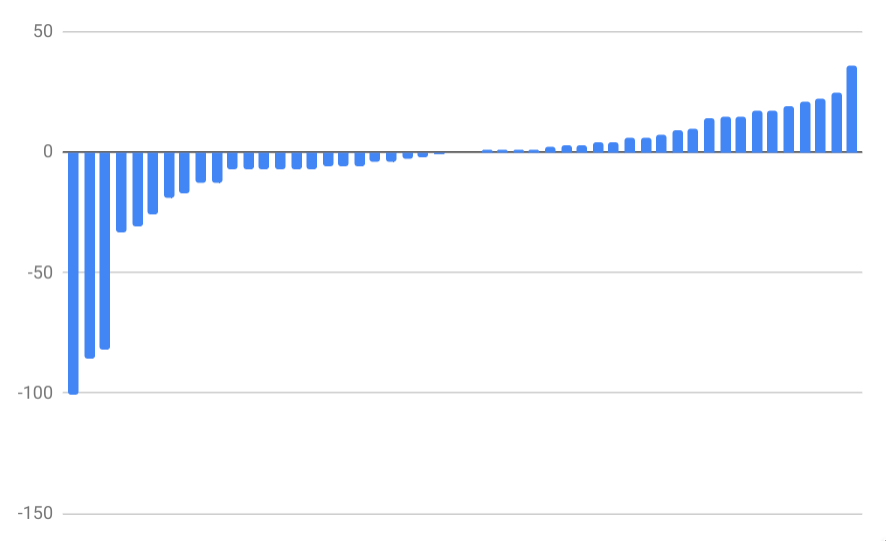
\includegraphics[scale=0.3]{random_vs_linear.png}
    \caption{random strategy vs. linear embedding RL}
  \end{subfigure}
  
  \begin{subfigure}[b]{0.5\textwidth}
    \centering
  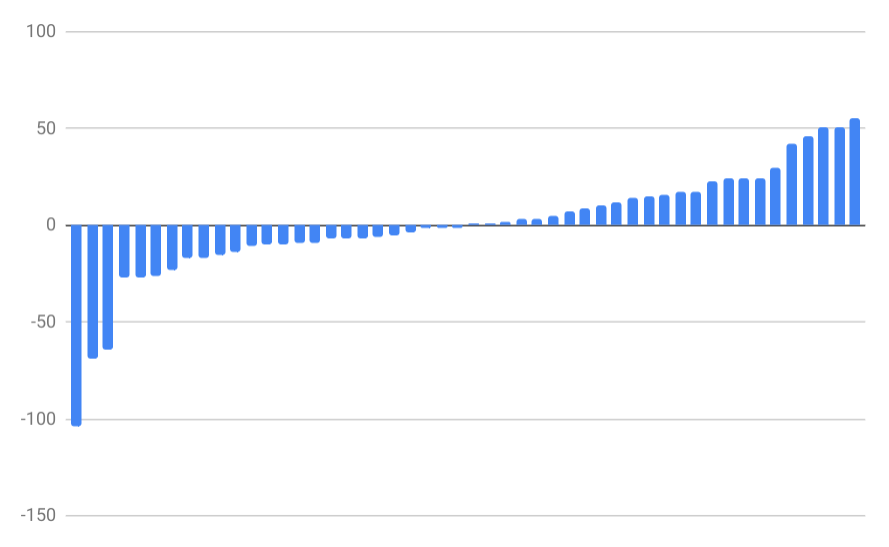
\includegraphics[scale=0.3]{random_vs_graph.png}
  \caption{random strategy vs. graph embedding RL}
  \end{subfigure}

  \caption{Detailed comparison of three models on 50 test instances.}
\end{figure}

\section{Related Work}

As artifical neural networks greatly succeeded in vision and natural language tasks in last ten years,
many works that combine deep learning and logical reasoning also has been emerged recently.
Some of the work are completely based on neural network, as opposed to utilizing
an existing deterministic framework. \citeauthor{selsam2018learning} proposed to 
use message-passing neural network to learn the assignment of a SAT problem \cite{selsam2018learning}.
We adapt a similar graph representation from \citeauthor{selsam2018learning}, but use it 
on DPLL, which poses a difficulty on handling dynamic graph strcuture.
Based on \citeauthor{selsam2018learning}'s NeuraSAT, a ICLR 2019 paper
further improves the model that directly generates the assignment in a unsupervised fashion, 
but works on circuit-sat problem\cite{anonymous2019learning}.

\section{Conclusion}

We investigate the problem of learning branching heuristics of SAT by 
graph neural networks and show the preliminary result. 
We note that since the random 3-SAT problems are not tightly constrained,
which means there may exist many satisfiable assignments, the numbers we showed
in Section 4 does not strictly imply the policy network has learned effective
branching heuristics. We leave the examination of ability of generalizing
on larger instances as future works. The graph currently experimented is still 
static, implementing and tweaking the dynamicaly updated GNN (as discussed in 
Section 2.2) is another on-going work.

\textbf{Acknowledgement} The author would like to thank Fei Wang for the inspiring discussion and 
help of the machine learning part.

\clearpage{}

% %% Acknowledgments
% \begin{acks}                            %% acks environment is optional
%                                         %% contents suppressed with 'anonymous'
%   %% Commands \grantsponsor{<sponsorID>}{<name>}{<url>} and
%   %% \grantnum[<url>]{<sponsorID>}{<number>} should be used to
%   %% acknowledge financial support and will be used by metadata
%   %% extraction tools.
%   This material is based upon work supported by the
%   \grantsponsor{GS100000001}{National Science
%     Foundation}{http://dx.doi.org/10.13039/100000001} under Grant
%   No.~\grantnum{GS100000001}{nnnnnnn} and Grant
%   No.~\grantnum{GS100000001}{mmmmmmm}.  Any opinions, findings, and
%   conclusions or recommendations expressed in this material are those
%   of the author and do not necessarily reflect the views of the
%   National Science Foundation.
% \end{acks}


%% Bibliography
\bibliography{reference}


%% Appendix
% \appendix
% \section{Appendix}

% Text of appendix \ldots

\end{document}
